\subsection{Universidad de Hong Kong - China}
Presentamos en la siguiente tabla los resultados obtenidos del último monitoreo.

\bigskip

\begin{tabular}{ | l | c | c | c | c |}
	\hline
		Hop & IP &  RTT promedio (s)  & deltaRTT promedio & Ubicación\\
 	\hline
		1  &  192.168.0.1  &  0.021503 &  0.021503 & Argentina - Buenos Aires \\
	\hline
		2  &  200.89.166.177  &  0.028651 &  0.007148 & Argentina - Buenos Aires\\
	\hline
		3  &  200.89.165.130  &  0.025739 &  0 & Argentina - Buenos Aires\\
	\hline
		4  &  200.89.165.222  &  0.031074 &  0.005334 & Argentina - Buenos Aires\\
	\hline
		5  &  208.178.195.205  &  0.02794 &  0 & Estados Unidos - Florida \\
	\hline
		6  &  67.17.106.162  &  0.1641088 &  0.136164 & Estados Unidos - Kansas \\
	\hline
		7  &  64.212.107.98  &  0.1607451 &  0 & Estados Unidos - Kansas \\
	\hline
		8  &  129.250.3.172  &  0.1631746 &  0.002429 & Estados Unidos - Colorado \\
	\hline
		9  &  129.250.2.219  &  0.1854111 &  0.022236 & Estados Unidos - Colorado\\
	\hline
		10  &  129.250.7.69  &  0.1903247 &  0.004913 & Estados Unidos - Colorado \\
	\hline
		11  &  129.250.2.177  &  0.307158 &  0.116833 & Estados Unidos - Colorado \\
	\hline
		12  &  129.250.6.144  &  0.313425 &  0.006267 & Estados Unidos - Colorado\\
	\hline
		13  &  129.250.2.222  &  0.366600 &  0.0531743 & Estados Unidos - Colorado\\
	\hline
		14  &  129.250.6.125  &  0.351373 &  0 & Estados Unidos - Colorado \\
	\hline
		15  &  129.250.3.11  &  0.3576226 &  0.006249 & Estados Unidos - Colorado\\
	\hline
		16  &  203.131.246.154 &  0.391269 &  0.0336466 & Hong Kong - Districto Central \\
	\hline
		17  &  115.160.187.110 &  0.387334 &  0 & Hong Kong - Districto Central\\
	\hline
		18  &  202.130.98.102  &  0.373508 &  0 & Hong Kong - Districto Central\\
	\hline
		19  &  203.188.117.130 &  0.380355 &  0.006846 & Hong Kong - Districto Central\\
	\hline
		20  &  202.14.80.153  &  0.378142 &  0 & Hong Kong - Districto Central\\
	\hline
		21  &  143.89.14.2  &  0.380775 &  0.002632 & Hong Kong - Districto Central\\
	\hline
		22  &  143.89.14.2  &  0.382564 &  0.001789 & Hong Kong - Districto Central\\
	\hline
		23  &  143.89.14.2  &  0.383357 &  0.000793 & Hong Kong - Districto Central\\
	\hline
		24  &  143.89.14.2  &  0.384837 &  0.001479 & Hong Kong - Districto Central\\
	\hline
		25  &  143.89.14.2  &  0.384046 &  0 & Hong Kong - Districto Central\\
	\hline
		26  &  143.89.14.2  &  0.385690 &  0.001644 & Hong Kong - Districto Central\\
\hline
\end{tabular}

\bigskip

En base a los resultados obtenidos tomamos los $Delta$ $RTT$ y realizamos un test de normalidad de nivel $alpha$ $0.005$ y podemos concluir que sigue una distribución Normal. \\

Además realizamos el Test de Grubbs para determinar la existencia de outliers, dichos valores representan a los saltos oceánicos, es decir cuando un paquete realiza un salto de un servidor situado en un continente distinto al del salto anterior.\\
El test nos dio $Rechadazo$, como era de esperarse, debido a que realizamos una consulta a una Universidad situada en el continente asiatico. Para sorpresa nuestra, detectamos outliers en los Hop 6 y 11. El número 11 efectivamente es un salto oceanico, ya que pasa de un router situado en $Estados Unidos$ a uno en $Hong Kong$. En cambio el número 6 es un salto desde $Argentina$ a $Estados Unidos$, debido a la distancia entre un router y otro nuestro test lo detecta como un salto oceánico, a pesar de no serlo.\\


\begin{figure}[H]
\centering
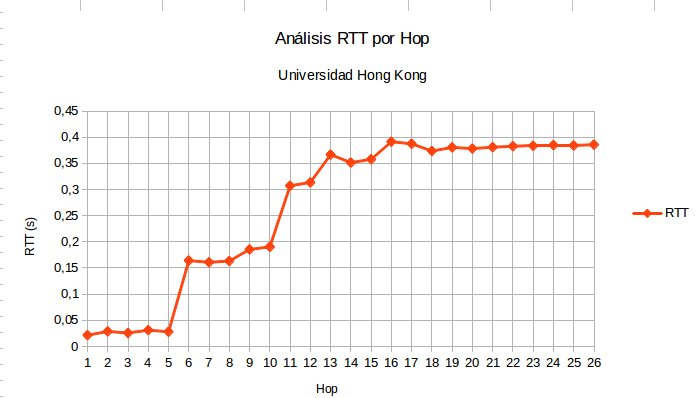
\includegraphics[width=1\textwidth]{graficos/rTT_HongKong.jpg}
\caption{RTT promedio por hop - Universidad de Hong Kong}
\label{hongkong_rtt}
\end{figure}

\begin{figure}[H]
\centering
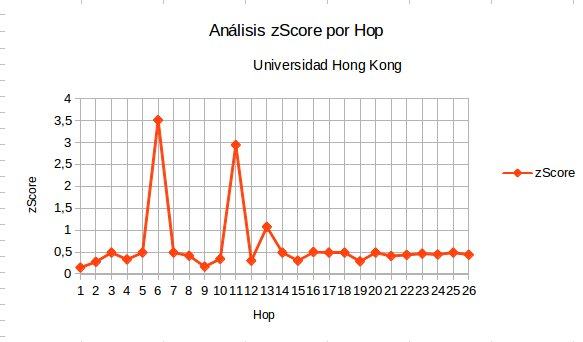
\includegraphics[width=1\textwidth]{graficos/zScore_HongKong.jpg}
\caption{zScore promedio por hop - Universidad de Hong Kong}
\label{hongkong_zs}
\end{figure}

A continuación hemos trazado en un mapa la ruta de nuestro host hasta el host destino ubicado en Hong Kong - China:
\begin{figure}[H]
\centering
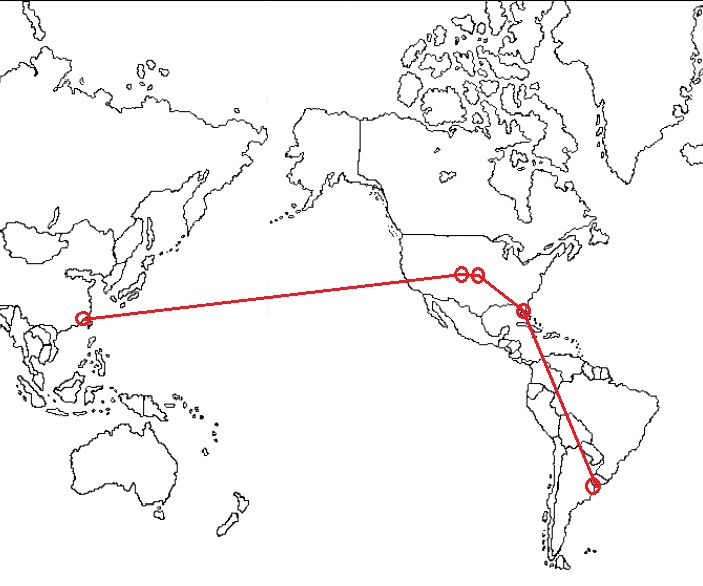
\includegraphics[width=0.8\textwidth]{graficos/mapa_hongKong.jpg}
\caption{Ruta en Internet - Universidad de Hong Kong}
\label{hongkong_zs}
\end{figure}
